\chapter[\diva\divaspace code]{\diva\divaspace code}
%-----------------------------
\hypertarget{DIVACODE}{}

\lettrine[lines=2]{T}{he} engine of \diva\, is a set of Fortran $77$ subroutines driven by local input \texttt{fort.*} files and local output \texttt{fort.*} files.

The GUI is driven by programs written in \hyperlink{TCL}{\tcltk}\, (see Sec. \ref{tclcode}).

This chapter is dedicated to the description of these programs, in order to allow the advanced user to adapt the code according to his needs.

\minitoc


\section[Fortran code]{Fortran code \expert}
%---------------------

The Fortran programs are sorted according to their purpose: Analysis, Mesh Generation, Graphical Interface, NetCDF and Utilities.

\subsection[\diva\divaspace programs]{\diva\divaspace programs [\texttt{src/Fortran/Calc}]}
%------------------------------------------------------------------------------------------

The main file of the Fortran code is \texttt{diva.f}: this routine calls the subroutines enumerated below, in order to perform a \diva\, analysis:
\vspace{.15cm}
\begin{description}
\item[\texttt{mathpr.f}]: describes the mathematical problem.
\item[\texttt{topolo.f}]: describes the topology of the finite element grid.
\item[\texttt{meshgn.f}]: generates a square finite element mesh on a regular grid.
\item[\texttt{datapr.f}]: input of data to be fitted by spline smoothing.
\item[\texttt{bcondi.f}]: Dirichlet boundary conditions to be fixed.
\item[\texttt{constr.f}]: input of information for constraint implementation.
\item[\texttt{solver.f}]: builds and solves the global linear finite element system.
\item[\texttt{stores.f}]: storage of the solution.
\item[\texttt{esterr.f}]: estimates the analysis error (same grid as the analysis).
\item[\texttt{coord.f}]: coordinate change (longitude, latitude) to $(x,y)$ and $(x,y)$ to (longitude, latitude) if requested.
\item[\texttt{gcvfac.f}]: estimates the analysis error by generalized cross-validation.  
\item[\texttt{dataqc.f}]: data quality check: estimates of expected data-analysis differences.   
\item[\texttt{covar.f}]: calculation of \diva\, kernel for subsequent error fields.        
\end{description}
\vspace{.15cm}
Other routines related to \diva\,calculation:
\begin{description}
\item[\texttt{allody.f}]: dynamical allocation of storage area in $S$ or $L$ vector.
\item[\texttt{bilinin.f}]: interpolates from a regular field into $xt,yt$; called in \texttt{constr.f}.
\item[\texttt{finca.f}]: finds in which region is one point.
\item[\texttt{optimi.f}]: subroutines used for the optimisation:

\begin{itemize}

\item[] \texttt{divesp.f}: subdivides the space for optimisation;
\item[] \texttt{sizes2.f}: computes the size of the space for elements of type 2;
\item[] \texttt{sizes3.f}: computes the size of the space for elements of type 3;
\item[] \texttt{repel2.f}: distributes the elements of type 2 in kntc table;
\item[] \texttt{repel3.f}: distributes the elements of type 2 in kntc table;
%\item \texttt{findca.f}: finds in which region is one point;
\item[] \texttt{locpt2opti.f}:  locates the $(x,y)$ point in the structure (for ityp=2);
\item[] \texttt{locpt3opti.f}:  locates the $(x,y)$ point in the structure (for ityp=3);
\item[] \texttt{sortdopti.f}:  sorts the data according to the sequence of elements;
\item[] \texttt{qs2i1r.f}:  quick Sort algorithm for \texttt{sortdopti} (from \url{www.netlib.org});
\item[] \texttt{calpsoopti}: computes pseudo data sets for error estimates;
\item[] \texttt{fcorropti.f}:  part of \texttt{calpsoopti};
\item[] \texttt{tabess.f}: tabulates the Bessel function for the calculation of error.
\end{itemize}


\item[\texttt{repeltest.f}]: called in \texttt{datapr.f}
\item[\texttt{shapef.f}]: evaluation of the shape functions at Gauss points.
\item[\texttt{utilit.f}]: utility routines.
\item[\texttt{uur.f}]: for the advection constraint.
\item[\texttt{uwrit2.f}]: writes the field $C(I,J,K)$.  
\item[\texttt{varl.f}]: for variable correlation length.
\item[\texttt{vtools.f}]: various subroutines: 
\begin{itemize}
\item[]  \texttt{intsec}: calculate center coordinates of quadrangular element;
\item[]  \texttt{istria}: check if one point lies inside a triangle;
\item[]  \texttt{prskyh}: print a vector to check.
\end{itemize}

\end{description}


\subsection[Mesh programs]{Mesh programs [\texttt{src/Fortran/Mesh}]}
%--------------------------------------------------------------------

Files related to the generation of coastlines:
\begin{description}
\item[\texttt{contourgen.f}]: check the format of an existing contour file (no repeated points, no crossing, contour not too fine).
\item[\texttt{contourgen.f}]: create contours based on topography;
\item[\texttt{coa2conf.f}]: go from ODV \texttt{.coa} files (see documentation of ODV) to \diva\, \texttt{coast.cont} files, using a resolution comparable to the specified gridded output of \texttt{divacalc}.
\end{description}

Files related to mesh generation:
\begin{description}
\item[\texttt{generopt.f}]: generate a multi-connex 2D mesh with the \textit{Delaunay tri\-angu\-la\-tion};
\item[\texttt{generopt4.f}]: same as generopt but in real*4 precision;
\item[\texttt{generopt8.f}]: same as generopt but in real*8 precision.
\end{description}


\subsection[Pipetest]{Pipetest [\texttt{src/Fortran/Pipetest}]}
% -----------------------------------------------------------

File \texttt{piperw.f} checks if \textit{pipe} is working within your \diva\,installation.

\subsection[Utilities]{Utilities [\texttt{src/Fortran/Util}]}
% -----------------------------------------------------------

\begin{description}
\item[\texttt{alpha.f}] computes the values of $\alpha_{0}$ and $\alpha_1$.

\item[\texttt{calcest.f}]: from relative weight on data points (data file \texttt{fort.44}) and generalized cross validator value (available in \texttt{./output/gcvval.dat}), produces the file containing the expected misfit value at data locations (\texttt{fort.76}), to be used by \texttt{look\-for\-outliers.a} for outliers detection. Used in \texttt{divaqcter}.

\item[\texttt{calcestbis.f}]: from relative weight on data points (data file \texttt{fort.44}) and the trace 
of the analysis matrix (available in \texttt{./\-output/\-gcvval.dat}) produces the file
containing the expected misfit value at data locations (\texttt{fort.76}), to be 
used by \texttt{look\-for\-outliers.a} for outliers detection. Used in \texttt{divaqcbis}.

\item[\texttt{calcmu.f}] computes the coefficient $\mu$ knowing  the characteristic length $L$ and the signal-to-noise ratio $\snr$.

\item[\texttt{cverror.f}]: rms error by cross validation (called in \texttt{divacvrand}).

\item[\texttt{cverroraii.f}]: same as \texttt{cverror.f} but using the \textit{missing-data lemma} (called in \texttt{divacv}).

\item[\texttt{cvtotalerror.f}]: sum of the different error contributions, in the resampling case (called in \texttt{divacvrand}).


\item[\texttt{datacheck.f}]: take the input data \texttt{./input/data.dat} and eliminates 
all data that fall outside the bounding box of the contours (called in \texttt{divadataclean}). 

\item[\texttt{datadiff.f}]: compute data anomaly (called in \texttt{divaanom})


\item[\texttt{dbdb2diva.f}]: converts topography extracted from Navy website into \diva\, compatible format (Sec. \ref{sec:toponavy}).

\item[\texttt{gebco2diva.f}]: converts topography extracted from GEBCO website into \diva\, compatible format (Sec. \ref{sec:topogebco}).


\item[\texttt{findmin.f}]: from a list of values (SNR, GCV, data-variance) found in \texttt{fort.11}, tries 
to find by local parabolic interpolation the minimum of GCV and the place SNR where it is found.

Points do not need to be ordered. Output (\texttt{fort.12}) contains the 
expected value of $\snr$ in which GCV is minimal as well as the \texttt{VARBAK} 
value. Used in \texttt{divagcv}.

Called in \texttt{divacv}, \texttt{divacvrand} and \texttt{divagcv}.


\item[\texttt{fitlsn.f}]: from the data file (\texttt{fort.10}) and information on coordinate change and 
reference field (\texttt{fort.11}), tries to fit the \textit{Bessel covariance function} to the data covariance (called in \texttt{divafit}).


Outputs:\\
\texttt{fort.66} contains the correlation length and an rough estimate of the signal-to-noise ratio;\\
\texttt{fort.99} contains the data-covariance over all distances;\\ 
\texttt{fort.98} contains the data covariance as a function of data-distance as well as the corresponding fit over distances up to the correlation length.

\item[\texttt{forgnuplot*.f}] consists in nine files for preparing the outputs to be viewed with the help of \gnuplot\,(see Sec. \ref{sec:visugnuplot}). 

\item[\texttt{griddef.f}] creates the file \texttt{GridInfo.dat}, of which the content is used for writing the NetCDF output.

%\item[\texttt{inversecont.f] allows one to reverse the 

\item[\texttt{lceleme.f}] computes the mesh characteristic length (called in \texttt{divacck} and \texttt{divamesh}).

\item[\texttt{lookforoutliers.f}] checks if there is outliers in the data provided for the analysis (called in \texttt{divacalc}, \texttt{divaqcbis} and \texttt{divaqcter}).

\item[\texttt{multiply.f}] does what its name says (called in \texttt{divarefe}).

\item[\texttt{subsampling.f}] creates a subsampling of the data (called in \texttt{dvsample}).

\item[\texttt{sumgrid.f}] performs the sum of two gridded fields in \gher\,format (called in \texttt{divasumup}).

\item[\texttt{sumup.f}] performs the sum element by element of two ascii files (called in \texttt{divasumup}).

\item[\texttt{topoprep.f}] makes easier the generation of the topography using a collection of local measurements (called in \texttt{divatopo}).

%\end{listept}
\end{description}

\paragraph{Remark:} grid definition for users is based on an origin which is the first grid point. 
In the code, \texttt{xori} and \texttt{yori} are defined by $x_i=$ \texttt{xori} $+i \Delta x$.
(and is thus shifted one grid space to the left compared to the user origin). Input file \texttt{fort.13} is modified from the \texttt{param.par} grid information by \texttt{griddef.a} accordingly, while \texttt{GridInfo.dat} contains the user grid as defined in \texttt{param.par}.

% -----------------------------------------------------------------------------------

\subsection[NetCDF output]{NetCDF output [\texttt{src/Fortran/NC}]}

Three files allow getting an output in NetCDF format \footnote{Do not forget you need the NetCDF library if you want to compile these files. The library needed by your system can be downloaded from\\
\url{http://www.unidata.ucar.edu/software/netcdf/}}
:\\ 
\texttt{netcdfoutputfield.f}, \texttt{netcdfoutputerror.f}, \texttt{netcdfoutput.f}. 

The two first routines write the analysed and the error fields in two different NetCDF files: \texttt{anlysed\_field.nc} and \texttt{error\_field.nc}. The last programs generates \texttt{results.nc} which contains both the analysis and the error fields. The information required for the coordinates (xorigin, y origin, dx, dy, xend, yend) are read from \texttt{GridInfo.dat}.

\begin{exfile}[H]
1\\
1\\
.5\\
 .5\\
100\\
100
\caption{GridInfo.dat}
\end{exfile}


\subsection[GUI programs]{GUI programs [\texttt{src/Fortran/Extensions}]}
%-------------------------------------------------------------------------

The graphical interface requires some particular routines:
\begin{description}
\item[\texttt{extract.f}]: interface to select or extract Data from MODB and MED formatted databases.
\vspace{.25cm}
\item[\texttt{fem3d.f}] is based upon a mesh file and a bathymetry file (regular grid in the \gher\, format); it creates a result file containing information to determinate if a mesh is in land or is sea, for a given depth.
\vspace{.25cm}
% -----------------------------------------------------------------------------------
\item[\texttt{concat.f}] is used to create the 3D file from the 2D files.
\item[\texttt{stiff.f}] generates the rigidity file (\texttt{fort.60}) in the 3D case.
\item[\texttt{mask.f}] masked the solution according to the bathymetry and the depth.
\item[\texttt{sum.f}] writes the sum of two fields (with same dimensions) in \gher\, format.
\item[\texttt{substref.f}] subtracts the reference field to the computed solution (only available when using the \textit{semi-normed} reference field).
\vspace{.25cm}
\item[\texttt{header2.f}] and \texttt{visu.f} are subroutines to visualize the data, the mesh and the solution (requires the \plplot\, library). Two versions of \texttt{visu.f} are provided: one is located in \texttt{diva-\divaversion/\-src/\-Fortran/\-PlPlot} and the other in \texttt{diva-\divaversion/\-src/\-Fortran/\-NoPlPlot}. The first can be compiled only if you have installed the \plplot\, library on your computer (for now, only under Linux).
\end{description}



% --------------------------------------------------------------------------------------------

\section{Input and output files}
%-------------------------------

The Fortran executables (files ending by \texttt{.a}) work with input and output \texttt{fort.*} files:

\boxed{\texttt{generopt.a}}		

%--------------
\begin{itemize}
%_-------------

  \item   reads as inputs:			\\
  	\texttt{fort.10}:			coast file, see example file with description, case of a square island in a square sea.	\\				
	 	\texttt{fort.11}:			the parameters required for the mesh generation.					
	\item 	produces as outputs:	\\							

%--------------------------
\begin{itemize}
%--------------------------

\item \texttt{fort.22}, which contains the finite element mesh: 
%---------------------------------------------------
\begin{enumerate}
%---------------------------------------------------

\item the first part of the file has three columns: the first column gives the numbers of the nodes; the second and third ones give the $x-$ and $y-$coordinates of the nodes, respectively. \\
\example first line indicates that node n$^{\circ}$ is located in $(-1,-1)$.
\item the second part is composed of only one column, which indicates the numbers of the interfaces;
\item the last part has six columns: columns 1, 3 and 5 specify the line numbers where the coordinates of the triangle points can be found; columns 2, 4 and 6 specify the interfaces numbers of the considered element.\\
\example the last line says that the last elements has its coordinates in lines 2, 3 and 5, \textit{i.e.}, at has points $(1,-1)$, $(1,1)$ and $(-0.333333343  0.333333343)$; it also says that this element is composed of interfaces n$^{\circ}$ 13, 8 and 12.

%---------------------------------------------------
\end{enumerate}
%---------------------------------------------------


%\begin{minipage}{.4\textwidth}{

\begin{exfile}[htpb]
\begin{footnotesize}
\texttt{1 -1. -1.\\
 9  1. -1.\\
 4  1.  1.\\
 10 -1.  1.\\
 7 -0.333333343  0.333333343\\
 5\\
 11\\
 6\\
 12\\
 8\\
 2\\
 13\\
 3\\
 3 -6 4 -7 5 -8\\
 4 -9 1 -10 5 -7\\
 1 -11 2 -12 5 -10\\
 2 -13 3 -8 5 -12\\
} 
\end{footnotesize}
\caption{fort.22\label{fig:fort22}}
\end{exfile}

%\end{minipage}
%\begin{minipage}{.6\textwidth}

\begin{figure}[H]
\centering
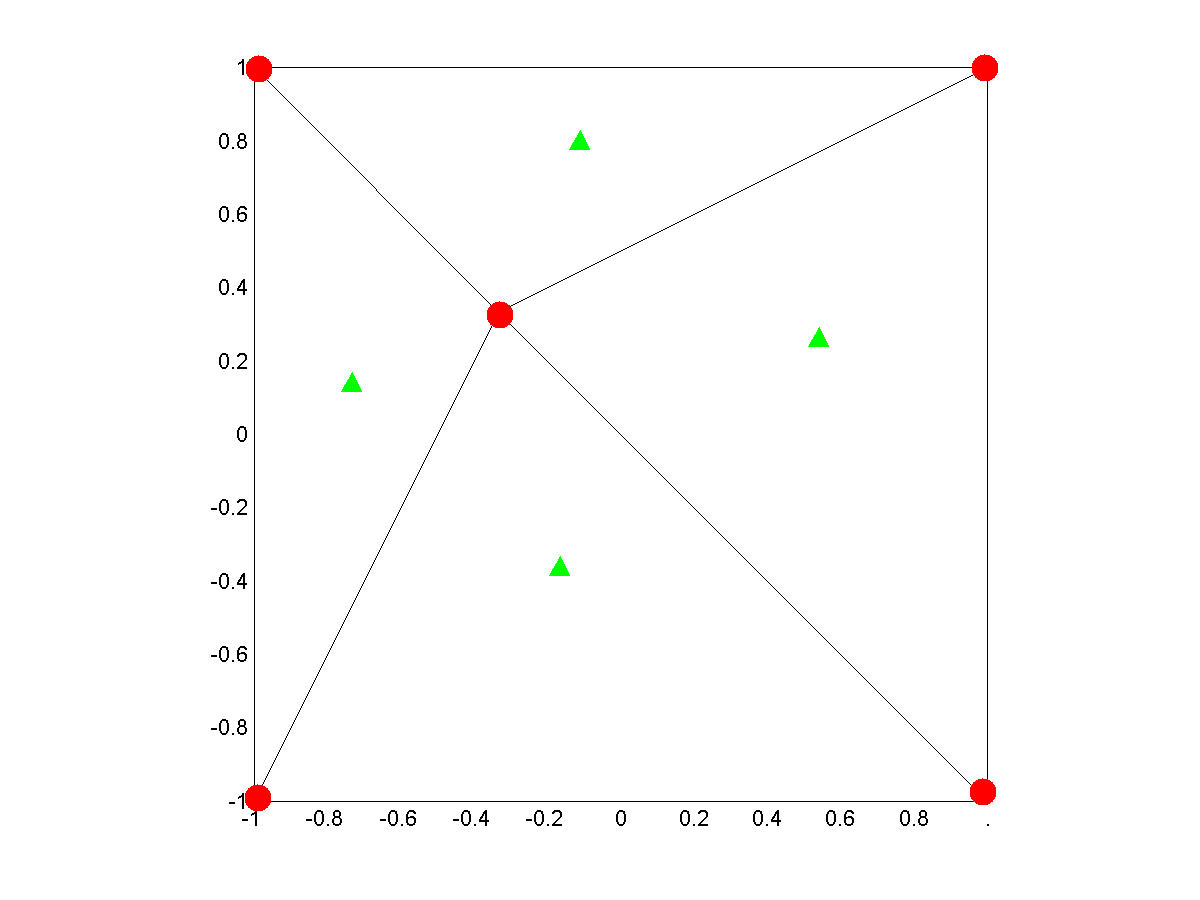
\includegraphics[width=.7\textwidth]{SimpleMesh_mesh}
\caption[Example of simple mesh]{Example of simple mesh corresponding to file \texttt{fort.22}}
\end{figure}

%\end{minipage}



\item \texttt{fort.23}, filled with topological parameters: 
\begin{enumerate}
\item total number of vertex nodes (red dots);
\item total number of interfaces (black lines);  
\item total number of elements (green triangles).
\end{enumerate}

\begin{exfile}[H]
%\begin{footnotesize}
\begin{verbatim}
 5
 8
 4
 \end{verbatim}
%\end{footnotesize}
\caption{fort.23\label{fig:fort23}}
\end{exfile}
 
\end{itemize}

\end{itemize}
%--------------------------------------------------------------------
\boxed{\texttt{diva.a}}
\begin{itemize}	
    \item reads as inputs: \\								
	 	\texttt{fort.10}:			\texttt{divawork} organizer, defining which modules to use and how, including several parameters.\\					
		\texttt{fort.11}:			finite element mesh, copy of the \texttt{fort.22} produced by \texttt{generopt.a}.\\					
	 	\texttt{fort.12}:			$\alpha_0$ and $\alpha_1$, calculated as: 
	 	\[\alpha_0=\frac{1}{L^{4}}\quad \textrm{and}  \quad  \alpha_1 =\frac{2}{L^{2}}.	\]				
	 	\texttt{fort.13}:			characteristics of regular output grid.\\					
		\texttt{fort.20}:			data file; 4 columns: $|X|Y|data(X,Y)|\mu|$, where  
		\[ \mu = 4\,\pi\,\frac{\snr}{L^{2}},\]
	  with $\snr$, the signal-to-noise ratio.	\\				
		\texttt{fort.79}:			coordinates where analyzed field values are requested; 2 columns separated by space: $|X|Y|$. \\					
	 	\texttt{fort.15}:			parameter \texttt{varbak}, variance of the background field, set as $=0$ will avoid calculating error field.				

\begin{exfile}[H]
coord 1\\
0\\
mathpr 1\\
2  -> ITYP\\
0  -> ISYM\\
2  -> IPB\\
topolo 1\\
 158 -> Number of Vertex Nodes\\
 426 -> Number of Interface Nodes\\
 268 -> Number of Elements\\
datapr 1\\
1\\
solver 1\\
0\\
stores 1\\
1  -> 1 if normal or seminormed final, otherwise 3\\
esterr 1\\
stopex\\
\caption{fort.10}
\end{exfile}
	  
	  
\begin{exfile}[H]
0.0001  -> alpha0\\
0.02  -> alpha1
\caption{fort.12}
\end{exfile}

\begin{exfile}[H]
0  0  -> xorigin, yorigin\\
1  1  -> dx, dy\\
100  100  -> nx, ny\\
-99999  -> Exclusion Value
\caption{fort.13}
\end{exfile}

\begin{exfile}[H]
\tt
90 90 1 12.5663706\\
90 80 1 12.5663706\\
90 70 1 12.5663706\\
$$\cdots$$\\
16 30 2 12.5663706\\
16 20 2 12.5663706\\
16 10 2 12.5663706
\caption{fort.20}
\end{exfile}
	  
  
	  
	  
\item produces as outputs:	\\							
\texttt{fort.71}:			field value at data points given in \texttt{fort.20}, ascii format.\\					
\texttt{fort.72}:			error value at data points given in \texttt{fort.20}, ascii format.\\					
\texttt{fort.73}:			error at points given in \texttt{fort.79}, ascii format.\\					
\texttt{fort.82}:			field value at points given in \texttt{fort.79}, ascii format.\\					
\texttt{fort.83}:			field on regular grid, ascii format.\\					
\texttt{fort.84}:			field on regular grid, gher format.\\					
\texttt{fort.86}:			error field on regular grid, ascii format.\\					
\texttt{fort.87}:			error field on regular grid, gher format.	
 				
\end{itemize}


\section[\tcltk\divaspace code]{\tcltk\divaspace code [\texttt{src/Tcl}]\label{tclcode}}
%---------------------------------------------------------------------------------------

The \tcltk\, files generate the graphical interface. The main file is \texttt{main.tcl}: it generates the main window, sets the paths to the \texttt{Tcl}, \texttt{GUIwork} and \texttt{bin} directories.

The different windows of the interface are created with the help of the following programs:
\begin{description}
\item [\texttt{menu.tcl}]: generates the menu bar for the Diva main menu, with its sub-menus: File, View, Options and Help;
\item[\texttt{data.tcl}]: builds the "Data" window (Diva/File/Data), which permits the data extraction;
\item[\texttt{fem.tcl}]: generates the finite elements mesh;
\item[\texttt{diva.tcl}]: performs the analysis on the data set; 
\vspace{.25cm}
\item[\texttt{view.tcl}]: defines the procedures for the visualization (menu Diva/View);
\item[\texttt{option.tcl}]: provides the sub-menu "Options" of the Diva main menu (Diva/Options);
\item[\texttt{help.tcl}]: builds the "Help" window in the Diva main menu (Diva/Help) and provides useful information about the meaning of the parameters choice and the interface.
\end{description}


The program \texttt{varlist.tcl} initializes the data in the dialogue boxes and the default access paths; \texttt{dictionary.tcl} is a dictionary in English and French; \texttt{tablist.tcl}: defines tables used in other subroutines.

%\item \texttt{edit.tcl}: defines the procedures \textcom{p\_copy}, \textcom{p\_paste} and \textcom{p\_cut} ;
\texttt{entry.tcl}, \texttt{misc.tcl} and \texttt{xmisc.tcl} define several procedures called in other \texttt{.tcl} files.


